\subsection{Bilan}

Notre bilan commence par la comptabilité des solutions VPN avec différent système d'exploitation.

\begin{figure}[H]
	\begin{center}
\begin{tabular}{|l|c|c|c|}
\hline
OS & Solution Windows & Solution Linux & Solution CISCO \\
\hline
Windows & Oui & Oui & Oui \\
Linux & Oui en théorie, Non en pratique & Oui & Oui \\
MAC (en théorie) & Oui & Oui & Oui \\
\hline
\end{tabular}
	\end{center}
	\caption{Compatibilité des OS}
	\label{Compatibilité_des_OS}
\end{figure}

D'un point de vue compatibilité OS, les solutions CISCO et OpenVPN repondent aux cahiers des charges. Il est à noter que nous n'avons pas pu tester nos différentes solutions sur MAC.

Afin de choisir la meilleure solution VPN, nous avons décider de mettre des notes sur allant de zero à cinq sur chacuns des critères que nous avons expliquer et de les regrouper dans un graphe en étoile.

Sur chaque graphe nous trouverons les critères suivants:
\begin{itemize}
 	\item Déploiement du serveur,
 	\item Bande passante effective,
 	\item Utilisation CPU,
 	\item Coût,
 	\item Stabilité de connexion,
 	\item Déploiement du client,
	\item Niveau de sécurité.
\end{itemize}



Commençons par la solution de Microsoft.


\begin{figure}[H]
	\begin{center}
		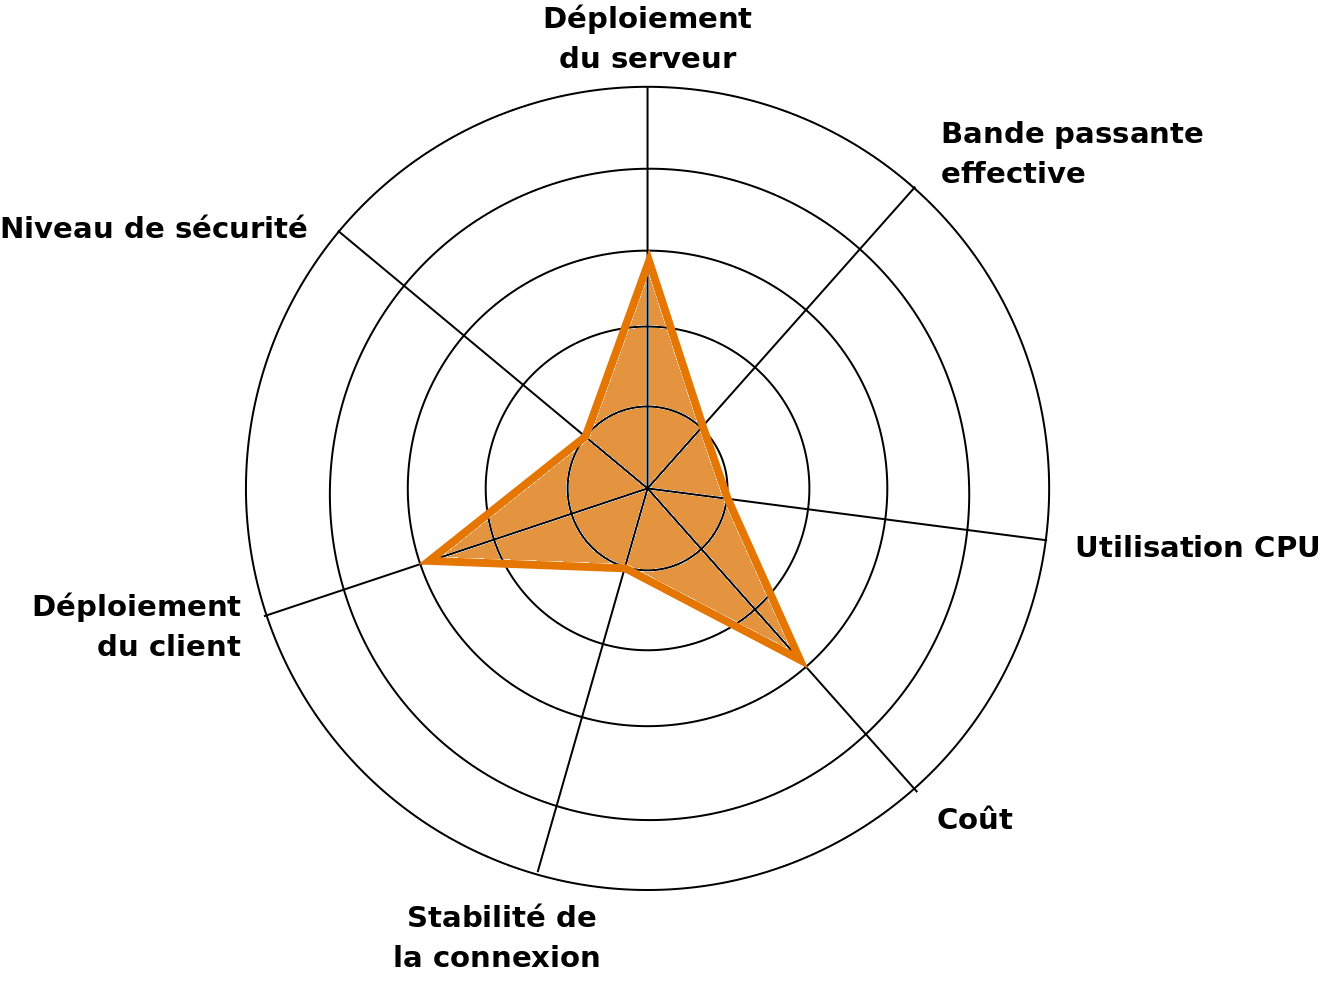
\includegraphics[width=0.75\textwidth]{partie_3/images/windows.png}\\
	\end{center}
	\caption{Graphe Windows}
	\label{Graphe Windows}
\end{figure}

En sommant les différents critères la solution de Microsoft a un résultat de \verb|13|


Voici le graphe pour la solution de CISCO

\begin{figure}[H]
	\begin{center}
		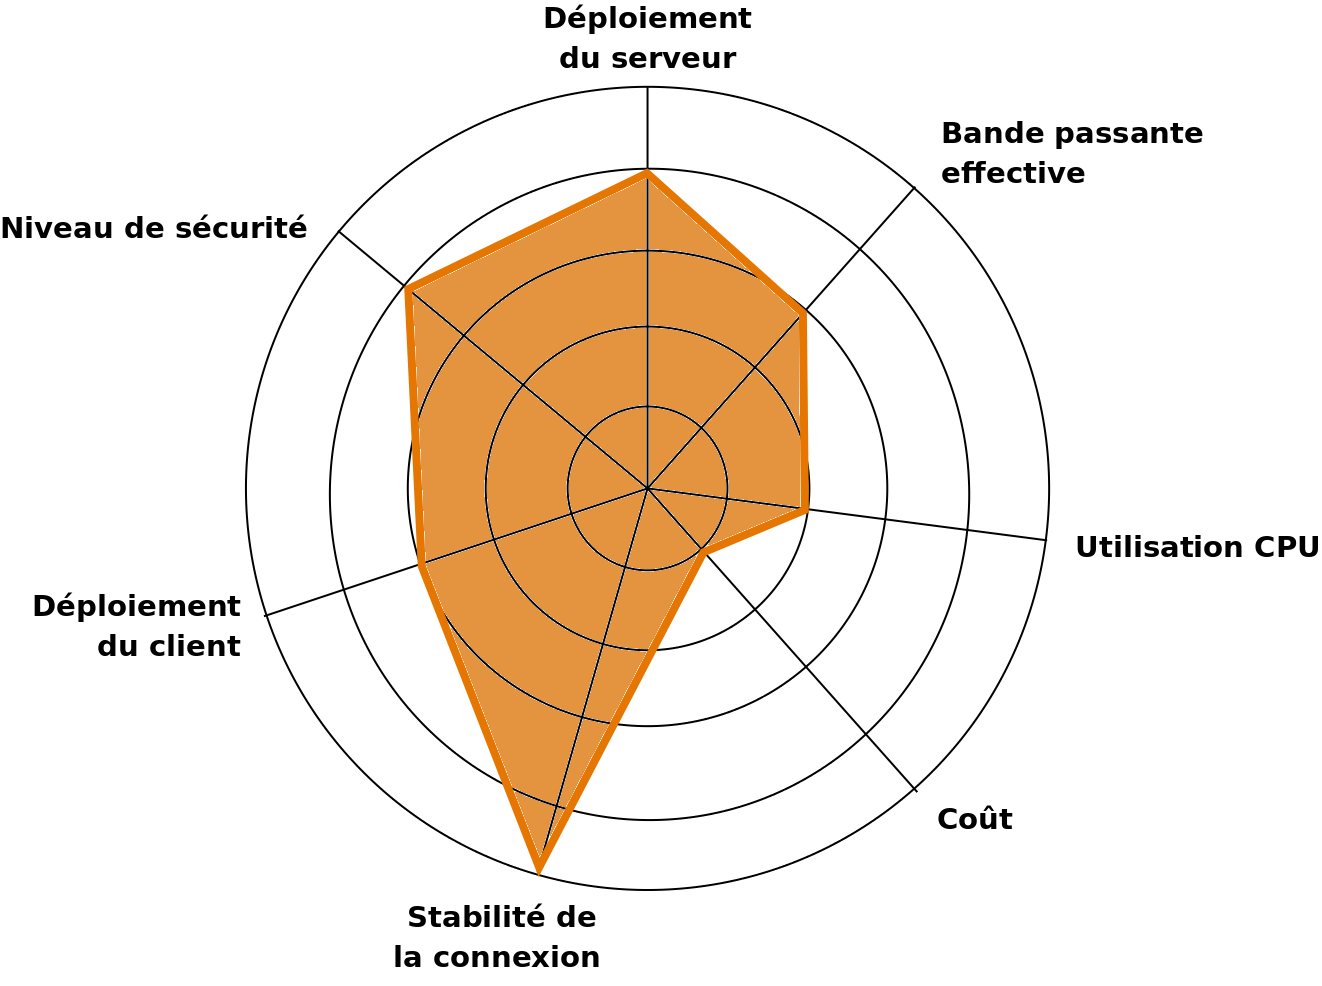
\includegraphics[width=0.75\textwidth]{partie_3/images/cisco.png}\\
	\end{center}
	\caption{Graphe Windows}
	\label{Graphe Windows}
\end{figure}

En sommant les différents critères la solution de Microsoft a un résultat de \verb|21|

Et pour terminer la solution OpenVPN

\begin{figure}[H]
	\begin{center}
		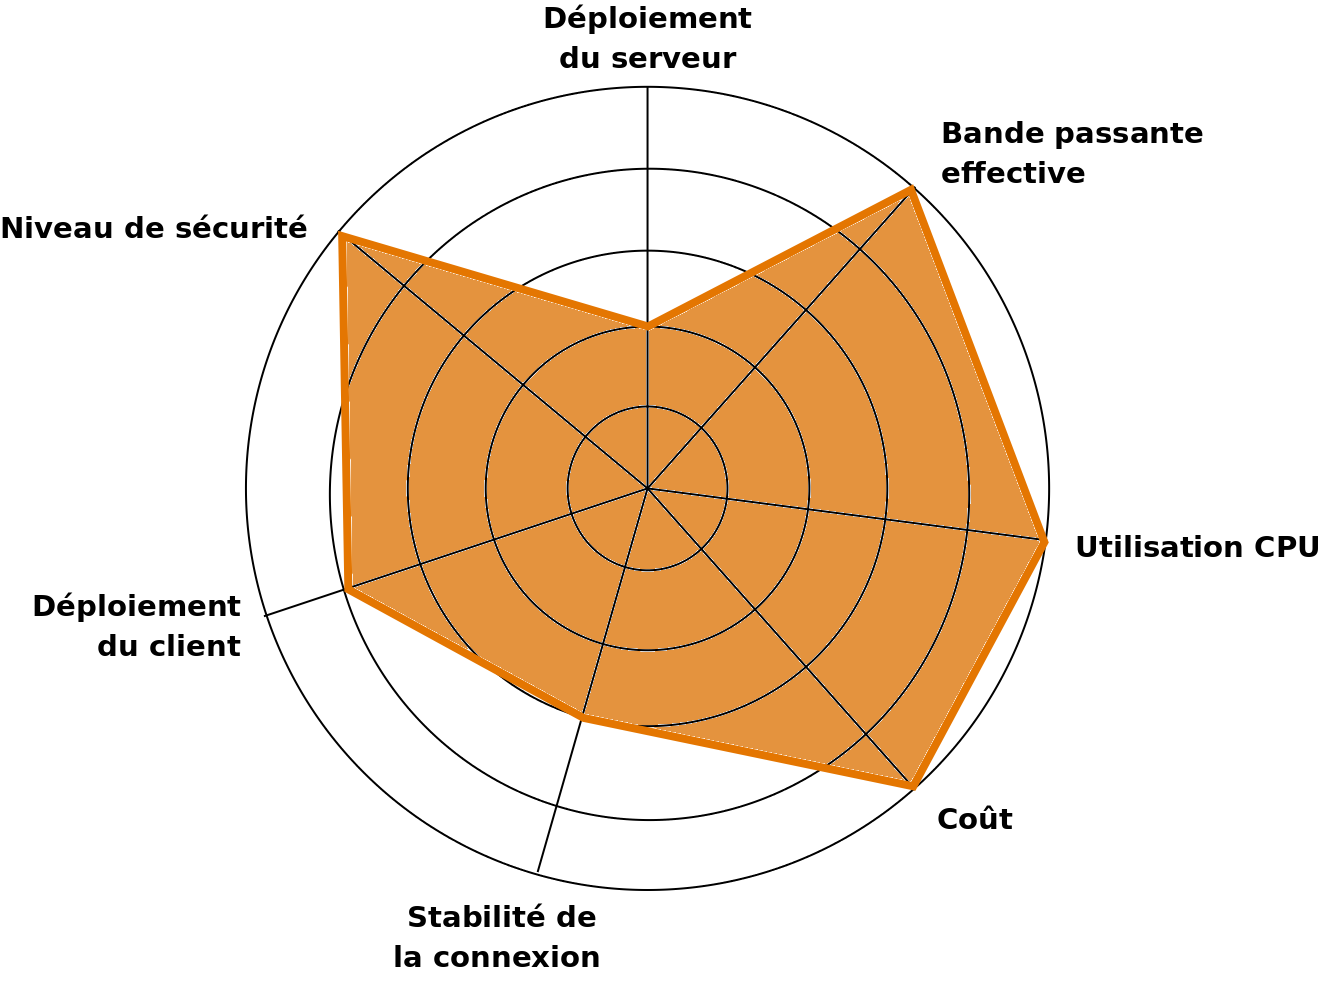
\includegraphics[width=0.75\textwidth]{partie_3/images/linux.png}\\
	\end{center}
	\caption{Graphe Windows}
	\label{Graphe Windows}
\end{figure}

En sommant les différents critères la solution de Microsoft a un résultat de \verb|29|


A la vue des différents graphes et à la compatibilité des solutions, nous pouvons conclure que la solution OpenVPN est la plus adaptée pour la mise ne place d'un VPN au sein de l'ISIMA.

